The frontend has been developed in Streamlit \cite{streamlit2018} in its latest version as of \today, 0.82.0 and can be accessed at \url{https://clustering.goethe.tech)}.
It provides a sidebar menu containing two dropdown lists. While the upper dropdown list can be used to select the dataset to be clustered, the second dropdown contains four different clustering algorithms to be applied: K-Means, Mean Shift, Spectral Clustering and Affinity Propagation. According to the selected clustering algorithm, the required input parameter can be set by dragging the slider on the respective widget. For this purpose, a message displays which kind of input parameter is required for the selected algorithm. 
Default values for different parameters vary with regard to the chosen dataset. We therefore provide slider widgets with different value ranges and varying default values according to the dataset to be clustered.
Once dataset and clustering technique are chosen, the \mintinline[bgcolor=code-bg]{python}{Calculate} button can be clicked to run the clustering procedure.
For convenience, selected dataset and algorithms are listed above the result part once again. After the dataset is clustered, a two-dimensional projection plot of all data points is displayed, distinguishing between different clusters with the help of distinct symbols and colors. 

In addition to that, we provide an evaluation module which can be used to compare different clustering strategies to each other. 

Our implementation is divided into segments to isolate clustering procedures from projecting the data into 2D and from visualizing the results.

Each of the clustering techniques that can be selected for grouping data points is implemented in a separate file which is named according to the technique. To run one of the clustering algorithms, the dataset has to be handed over in form of an n x m matrix consisting of n data points with m features. Moreover, a value for the algorithm specific parameter has to be provided. The \mintinline[bgcolor=code-bg]{python}{returns} parameter can be used to defined what output format is expected. We provide the possibility to distinguish between returning the fitted estimator, an n x (m+1) - matrix consisting of n data points with m features and a column containing a label for each data point or an n x 1 vector, which only includes a label for each data point. Running the clustering in its default mode, each technique returns the n x 1 label vector.
For the K-Means algorithm, the additional parameter state can be chosen. This value is used to initialize the random number generator such that always the same results are yielded \cite{sklearn_api}.\newline
In the \mintinline[bgcolor=code-bg]{python}{app.py} file, we implement all the functionalities concerning the frontend elements as well as choice of dataset and clustering technique. After reading the four different datasets using the \mintinline[bgcolor=code-bg]{python}{read_csv} method provided by pandas \cite{reback2020pandas, mckinney-proc-scipy-2010}, we calculate a cached version of the datasets projected into 2D to speed up all the following interactions. 
To project the datasets into 2D, we make use of the t-distributed Stochastic Neighbor Embedding (t-SNE) method provided by sklearn \cite{sklearn_api}. \mintinline[bgcolor=code-bg]{python}{t-SNE} is a method that facilitates displaying high-dimensional data in a 2D or 3D plot and nevertheless preserving local and global structures. This is done converting Euclidean distances between all data points in high dimensions into conditional probabilities such that high probabilities are allocated to similar data points while dissimilar data points are assigned a low probability. Afterwards, the same is done for all the data points projected into lower dimensions. The optimal projection of high-dimensional data points is finally found by minimizing the mismatch between calculated probabilities between points in high and in low dimensions\cite{tSNE}.\newline
As described earlier, we not only provide dropdown lists to enable the choice of a dataset as well as a clustering technique, but also adapt the slider widget label according to the required input parameter for the chosen algorithm. We define parameter value ranges along with default values appropriate to the chosen dataset. 
To run the clustering procedure, we implement an event handler checking for click events on the Calculate button. According to the selected clustering algorithm, we call the respective clustering function and hand over the dataset as an n x m matrix as well as the technique specific parameter value which was selected with the help of the slider widget.
In order to plot the resulting clusters, we call the \mintinline[bgcolor=code-bg]{python}{plot_tsne_2} function which we, again, implement in a separate file. In this method, we define a variety of symbols and colors to be able to distinguish between different clusters. For each data point, we check which cluster it was assigned to and connect it to the respective symbol and color. We finally create the plot showing the 2D clusters with the help of the Matplotlib visualization function \mintinline[bgcolor=code-bg]{python}{pyplot} \cite{Hunter:2007}.\\
Some screenshots like image \ref{img:frontend_screenshot_1} with explanation etc. 
\begin{figure}[H]
\caption{Frontend example screenshot}
%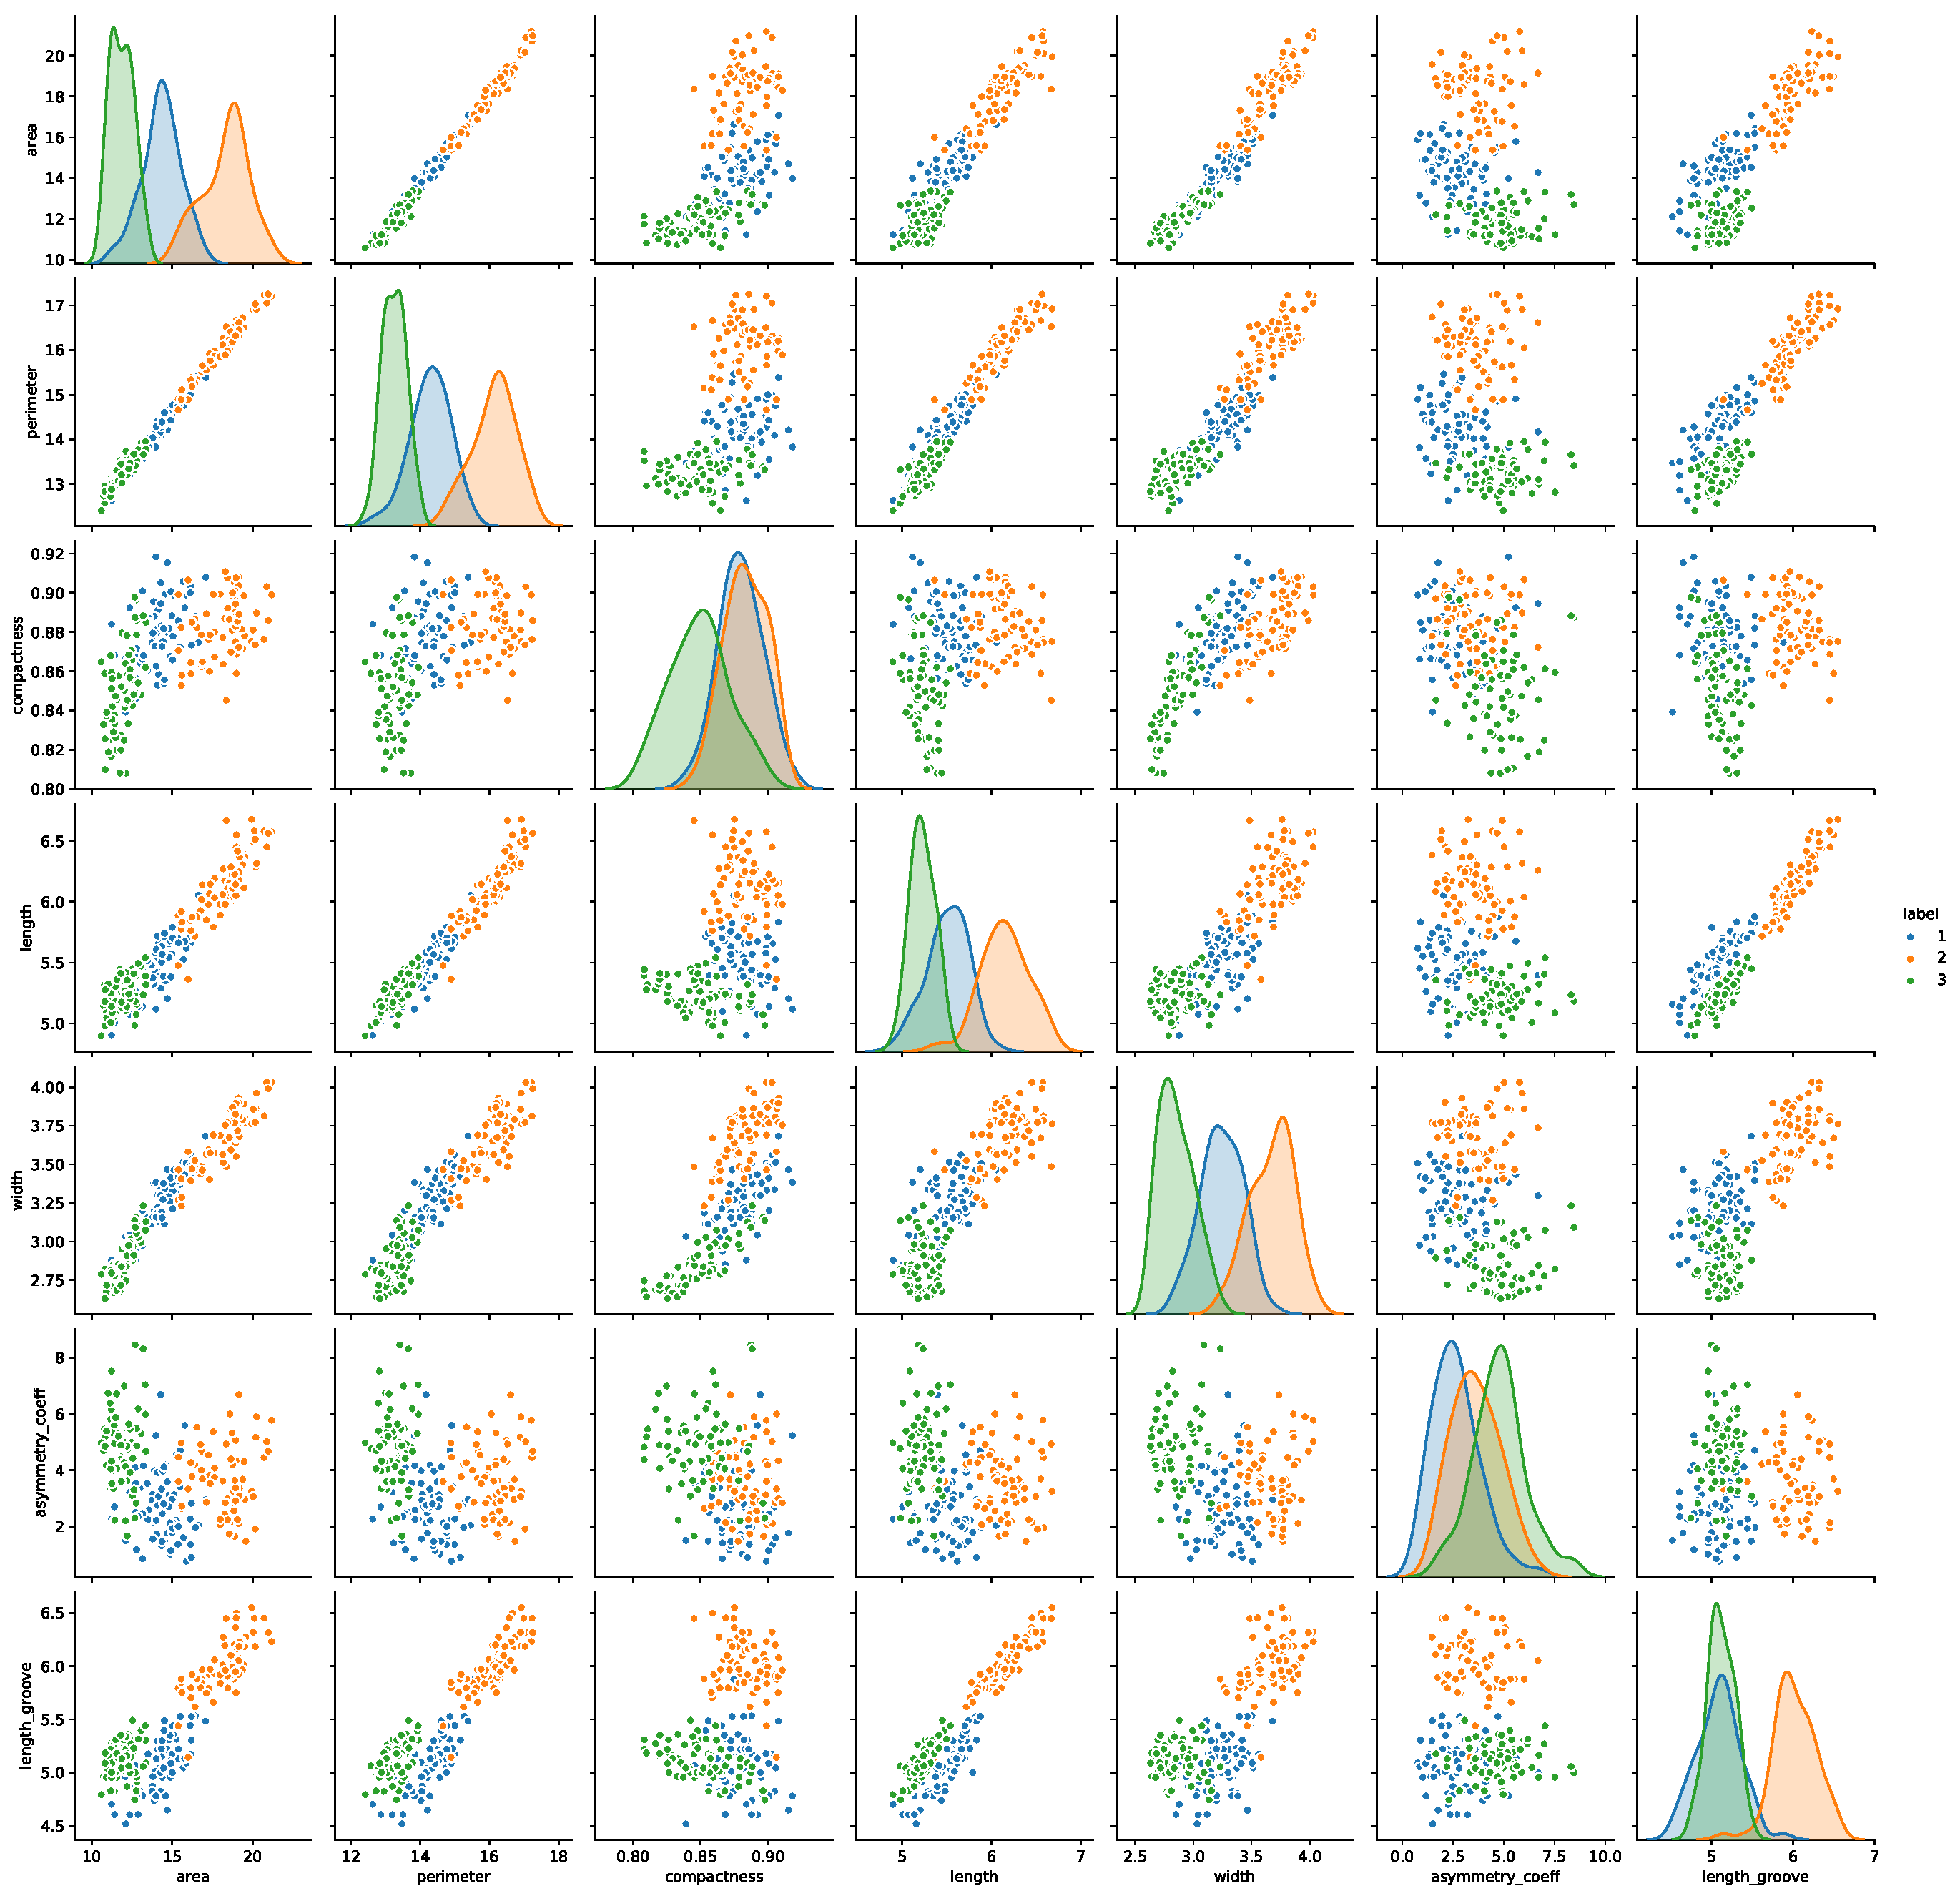
\includepdf[pages=-,scale=.4]{images/seeds_pairplot.pdf}
\begin{center}
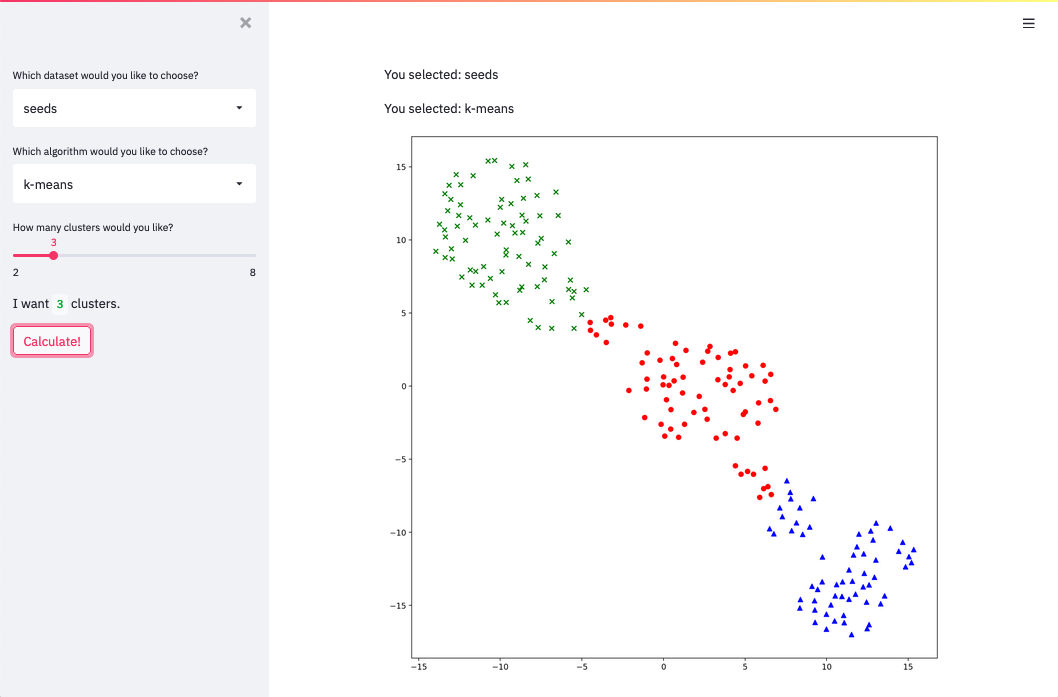
\includegraphics[width=0.75\textwidth]{images/frontend_beta_001.png}
\end{center}
\label{img:frontend_screenshot_1}
\end{figure}